\documentclass[aspectratio=169,xcolor={dvipsnames,table}]{beamer}
\usepackage[no-math,deluxe,haranoaji]{luatexja-preset}
\renewcommand{\kanjifamilydefault}{\gtdefault}
\renewcommand{\emph}[1]{{\upshape\bfseries #1}}
\usetheme{metropolis}
\metroset{block=fill}
\setbeamertemplate{navigation symbols}{}
\usecolortheme[rgb={0.7,0.2,0.2}]{structure}
%%%%%%%%%%%%%%%%%%%%%%%%%%%
%% さまざまなアイコン
%%%%%%%%%%%%%%%%%%%%%%%%%%%
\usepackage{fontawesome}
%%%%%%%%%%%%%%%%%%%%%%%%%%%
\usepackage{tikz}
\usepackage{xcolor}
\usepackage{circledsteps}
\usetikzlibrary{backgrounds}
\usepackage{tcolorbox}
\usepackage{tikzpeople}
\usepackage{twemojis}
\usepackage{tikzsymbols}
\usepackage{utfsym}\usepackage{figchild}
\usepackage{tikzlings}
\usepackage{scsnowman}
%%%%%%%%%%%%%%%%%%%%%%%%%%%
%% 場合分け
\usepackage{cases}
%%%%%%%%%%%%%%%%%%%%%%%%%%%
% \myAnch{<名前>}{<色>}{<テキスト>}
% 指定のテキストを指定の色の四角枠で囲み, 指定の名前をもつTikZの
% ノードとして出力する. 図には remember picture 属性を付けている
% ので外部から参照可能である.
\newcommand*{\myAnch}[3]{%
  \tikz[remember picture,baseline=(#1.base)]
    \node[draw,rectangle,line width=1pt,#2] (#1) {\normalcolor #3};
}
%%%%%%%%%%%%%%%%%%%%%%%%%%%%
%%%%%%%%%%%%%%%%%%%%%%%%%%%
%% 音声リンク表示
\newcommand{\myaudio}[1]{\href{#1}{\faVolumeUp}}
%%%%%%%%%%%%%%%%%%%%%%%%%%%
% \myEmph コマンドの定義
\newcommand{\myEmph}[3]{%
    \textbf<#1>{\color<#1>{#2}{#3}}%
}
%%%%%%%%%%%%%%%%%%%%%%%%%%
%% Change alert block colors
%%% 1- Block title (background and text)
\setbeamercolor{block title alerted}{fg=mDarkTeal, bg=mLightBrown!45!yellow!45}
\setbeamercolor{block title example}{fg=magenta!10!black, bg=mLightGreen!70}
%%% 2- Block body (background)
\setbeamercolor{block body alerted}{bg=mLightBrown!25}
\setbeamercolor{block body example}{bg=mLightGreen!15}
%%%%%%%%%%%%%%%%%%%%%%%%%%%
\title{English is fun.\,\,{}---主語と動詞---}
\author{}
\institute[]{}
\date[]

%%%%%%%%%%%%%%%%%%%%%%%%%%%%
%% TEXT
%%%%%%%%%%%%%%%%%%%%%%%%%%%%
\begin{document}
%%%%%%%%%%%%%%%%%%%%%%%%%%%%%%%
\begin{frame}[plain,label=title]
  \titlepage
\end{frame}
%%%%%%%%%%%%%%%%%%%%%%%%%%%%%%%
%%%%%%%%%%%%%%%%%%%%%%%%%%%%
\begin{frame}[plain]{Quiz 1}
 \large
\visible<1->{%
これからアルファベットを6つ順番に読みあげます。
聞こえたアルファベットを順番に小文字で書いてください。すると単語になります。その意味を表す図を選んでください
}
\mbox{}\hfill\visible<1->{\myaudio{./audio/quiz/quiz_a.mp3}}

\bigskip

\centering
\begin{tabular}{c@{   }c@{   }c@{   }c}
\scalebox{.8}{
\begin{tikzpicture}
\bear
\end{tikzpicture}%
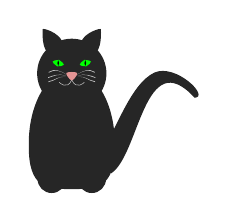
\begin{tikzpicture}
 \cat[eye=green]
\end{tikzpicture}}&
\scsnowman[scale=5,eyes, mouth,
nose, arms, hat=NavyBlue, muffler=Maroon,
buttons, snow, broom]&
\scalebox{6}{\twemoji{sushi}}&
\scalebox{6}{\twemoji{lemon}}\\
(a)&(b)&(c)&(d)
\end{tabular}

\bigskip

\Huge

\onslide<2->{a}%
\onslide<3->{n}%
\onslide<4->{i}%
\onslide<5->{m}%
\onslide<6->{a}%
\onslide<7->{l}%

\large
\mbox{}\hfill\visible<1->{\myaudio{./audio/quiz/answer_a.mp3}}

\end{frame}
%%%%%%%%%%%%%%%%%%%%%%%%%%%%
\section*{授業の流れ}
\begin{frame}[plain]
  \frametitle{授業の流れ}
  \tableofcontents
\end{frame}

\section{復習(アルファベット)}
%%%%%%%%%%%%%%%%%%%%%%%%%%%%%%
%\subsection{アルファベットのまとめ}
\begin{frame}[plain,label=matome]{アルファベットのまとめ}
  \begin{exampleblock}{Topics for Today}
\small
\pause
\begin{itemize}
 \item アルファベットは26種類です\pause
 \item 大文字と小文字があります\pause
       \begin{itemize}
	\item 大文字小文字を区別して書けるようになろう\pause
        \item 大文字を使うのは\pause
              \begin{itemize}
	       \item 文の先頭\pause
	       \item 人名\pause
	       \item \textrm{I}\,\,(わたし)はいつでも\pause
	      \end{itemize}
       \end{itemize}
 \item 聞き取れるようになったら実際に発音してみよう
\end{itemize}
      \end{exampleblock}
\end{frame}



\section{主語と動詞}

\begin{frame}<1-6>[plain, label=cats]{だれが何をしていますか}
\large

%\raggedleft
\begin{columns}
\begin{column}{.245\textwidth}
\visible<1->{この写真では}%

\bigskip

\visible<3->{ねこが}\\
\visible<4->{ミルクを\\飲んでいる}
\bigskip

\bigskip

\visible<5->{$\text{主語}=\text{ねこ}$}
\visible<6->{$\text{動詞}=\text{飲んでいる}$}
\end{column}
\begin{column}{.74\textwidth}
\includegraphics[width=.99\textwidth]{../images/cat_drinkimg_milk.jpg}
\end{column}
\end{columns}

\tiny
\raggedleft

"Domestic cat drinkimg milk" by Kengee8 is licensed under CC BY-SA 4.0.\\
 To view a copy of this license, 
visit \url{https://creativecommons.org/licenses/by-sa/4.0/?ref=openverse}.
\end{frame}



\begin{frame}<1-15>[plain,label=what_is_sv]{「主語」とは、「動詞」とは}
\large

\visible<1->{\alt<1>{\myAnch{syugo}{white}{だれだれは}}{\myAnch{SYUGO}{Maroon}{だれだれは}}\alt<1>{\myAnch{doshi}{white}{〜する}}{\myAnch{DOSHI}{NavyBlue}{〜する}}}
\bigskip

\visible<3->{\begin{enumerate}
 \item \alt<3>{\myAnch{s_1}{white}{わたしは}}{\myAnch{S_1}{Maroon}{わたしは}}英語を\alt<3-4>{\myAnch{v_1}{white}{話す}}{\myAnch{V_1}{NavyBlue}{話す}}。%
\hfill{}\visible<12->{hanas\textcolor{NavyBlue}{\bfseries u}}
 \item \alt<3-5>{\myAnch{s_2}{white}{あなたは}}{\myAnch{S_2}{Maroon}{あなたは}}寿司を\alt<3-6>{\myAnch{v_2}{white}{食べる}}{\myAnch{V_2}{NavyBlue}{食べる}}。%
\scalebox{2}{\twemoji{sushi}}%
\hfill{}\visible<13->{taber\textcolor{NavyBlue}{\bfseries u}}
 \item \alt<3-7>{\myAnch{s_3}{white}{われわれは}}{\myAnch{S_3}{Maroon}{われわれは}}バスで職場に\alt<3-8>{\myAnch{v_3}{white}{行く}}{\myAnch{V_3}{NavyBlue}{行く}}。\usym{1F68C}%
\hfill{}\visible<14->{ik\textcolor{NavyBlue}{\bfseries u}}
 \item \mbox{}\hspace{5pt}毎朝、\alt<3-9>{\myAnch{s_4}{white}{彼らは}}{\myAnch{S_4}{Maroon}{彼らは}}コーヒーを\alt<3-10>{\myAnch{v_4}{white}{飲む}}{\myAnch{V_4}{NavyBlue}{飲む}}。\scalebox{1.6}{\Coffeecup}%
\hfill{}\visible<15->{nom\textcolor{NavyBlue}{\bfseries u}}
\end{enumerate}}


\mbox{}\hfill \visible<1->{\myAnch{S}{Maroon}{主語}\myAnch{V}{NavyBlue}{動詞}}\end{frame}

%%%%%%%%%%%%%%%%%%%%%%%%%%%%%%%%%%%%%%%%%%%%%%
\begin{frame}<1-32>[plain,label=example_1]\frametitle{だれだれは〜する.}
 % \setbeamercovered{transparent}
  \begin{enumerate}
   \item<1-> \alt<14->{\Circled[outer color=Maroon]{I}}{I}  \alt<15->{\Circled[outer color=NavyBlue]{have}}{have} a car. \onslide*<2-25>{わたしは車を持っている。}\hfill\onslide*<27->{\footnotesize have: 持つ car: 車}
   \item<3->  \alt<16->{\Circled[outer color=Maroon]{We}}{We}  \alt<17->{\Circled[outer color=NavyBlue]{go}}{go} to work by bus. \onslide*<4-25>{われわれはバスで職場に行く。}\hfill\onslide*<28->{\footnotesize go: 行く work: 職場 by bus: バスで}
   \item<5->  \alt<18->{\Circled[outer color=Maroon]{They}}{They}  \alt<19->{\Circled[outer color=NavyBlue]{speak}}{speak} English and Japanese. \onslide*<6-25>{彼らは英語と日本語を話す。}\hfill\onslide*<29->{\footnotesize speak: 話す}
   \item<7->  \alt<20->{\Circled[outer color=Maroon]{I}}{I}  \alt<21->{\Circled[outer color=NavyBlue]{drink}}{drink} coffee every morning. \onslide*<8-25>{わたしは毎朝コーヒーを飲みます。}\hfill\onslide*<30->{\footnotesize drink: 飲む coffee: コーヒー every morning: 毎朝}
   \item<9->  \alt<22->{\Circled[outer color=Maroon]{They}}{They}  \alt<23->{\Circled[outer color=NavyBlue]{study}}{study} at the library. \onslide*<10-25>{彼らは図書館で勉強します。}\hfill\onslide*<31->{\footnotesize study: 勉強する at the library: 図書館で}
   \item<11->  \alt<24->{\Circled[outer color=Maroon]{We}}{We}  \alt<25->{\Circled[outer color=NavyBlue]{eat}}{eat} bread for breakfast. \onslide*<12-25>{われわれは朝食にパンを食べる。}\hfill\onslide*<32->{\footnotesize eat: 食べる bread: パン for breakfast: 朝食に}
  \end{enumerate}

\bigskip

\begin{exampleblock}<26->{Topic for Today}
  英文の骨格は主語と動詞です
     \end{exampleblock}

% Embed the sound file
\onslide<1->{%
\myaudio{./audio/003_sv_01.mp3}
}%
\hfill{}%
\onslide<32->{%
\myaudio{./audio/003_sv_02.mp3}
}
\end{frame}
%%%%%%%%%%%%%%%%%%%%%%%%%%%%%%%%%%%%%%%%%%%%%%
%\againframe{title}
%\againframe<6>{cats}
%\againframe<15>{what_is_sv}
%\againframe<13->{example_1}
%%%%%%%%%%%%%%%%%%%%%%%%%%%%%%%%%%%%%%%%
\section{主語と動詞の順番}
\begin{frame}[plain]\frametitle{だれだれは〜する.}
 % \setbeamercovered{transparent}

\begin{columns}
\begin{column}[t]{.45\textwidth}
\begin{block}{日本語}
わたしは英語を話します。\pause

英語をわたしは話します。\pause

英語を話します、わたしは。\pause

英語を話します。
\end{block}
\end{column}
\pause
\begin{column}[t]{.45\textwidth}
\begin{alertblock}{英語}
I speak English.\pause

\mbox{}\hspace{75pt}*I English speak\pause

\mbox{}\hspace{75pt}*Speak English I.\pause

\mbox{}\hspace{75pt}*Speak English.\pause

\scriptsize
\mbox{}\hspace{75pt}%
`*'は誤った文という記号 
\end{alertblock}
\end{column}
\end{columns}


\bigskip
\pause
\begin{exampleblock}{Topics for Today}
\begin{itemize}
 \item   英文の骨格は主語と動詞です
 \item   英語は語順がだいじです
 \item   英文にはかならず主語が必要
\end{itemize}
     \end{exampleblock}
\end{frame}


\subsection{まとめ}
\begin{frame}[plain]{まとめ}
 \begin{exampleblock}{Topics for Today}
\begin{itemize}
 \item   英文の骨格は主語と動詞です
 \item   英語は語順がだいじです
 \item   英文にはかならず主語が必要
\end{itemize}
     \end{exampleblock}
\end{frame}




\begin{frame}[plain]\frametitle{Exercises}
日本語を参考にして、主語と動詞を指摘してください。
\begin{enumerate}
    \item \alt<2->{\Circled[outer color=Maroon]{You}}{You} \alt<3->{\Circled[outer color=NavyBlue]{have}}{have} a nice car. あなたはいい車を持っている。
 \item \alt<4->{\Circled[outer color=Maroon]{I}}{I} \alt<5->{\Circled[outer color=NavyBlue]{play}}{play} the piano. わたしはピアノを弾きます。
    \item \alt<6->{\Circled[outer color=Maroon]{They}}{They} \alt<7->{\Circled[outer color=NavyBlue]{watch}}{watch} TV. 彼らはテレビを見ます。
    \item \alt<8->{\Circled[outer color=Maroon]{We}}{We} \alt<9->{\Circled[outer color=NavyBlue]{study}}{study} English. わたしたちは英語を勉強します。
 \item \alt<10->{\Circled[outer color=Maroon]{I}}{I} \alt<11->{\Circled[outer color=NavyBlue]{write}}{write} a letter. わたしは手紙を書きます。
     \item \alt<12->{\Circled[outer color=Maroon]{Birds}}{Birds} \alt<13->{\Circled[outer color=NavyBlue]{sing}}{sing}. 鳥は歌います。
    \item \alt<14->{\Circled[outer color=Maroon]{Dogs}}{Dogs} \alt<15->{\Circled[outer color=NavyBlue]{swim}}{swim} well. 犬はじょうずに泳ぎます。
     \item \alt<16->{\Circled[outer color=Maroon]{They}}{They} \alt<17->{\Circled[outer color=NavyBlue]{like}}{like} music. 彼らは音楽が好きです。
\end{enumerate}

% Embed the sound file
\onslide<1->{%
\myaudio{./audio/003_sv_03.mp3}
}
\end{frame}

%%%%%%%%%%%%%%%%%%%%%%%%%%%%%%%
\begin{frame}{}
\Huge

\centering

English is fun.
\end{frame}

\section*{See you next time.}
%\begin{frame}{}
%\phantomsection
%\end{frame}
\end{document}
